\chapter{Preliminaries:\\ Literature Review} \label{Chp: Literature Review}

In this chapter we review some literatures related to the security of WSNs in three aspects:
\begin{enumerate}
	\item Protocol and implementation flaws
	\item Traffic analysis techniques
	\item Information leakage detection
\end{enumerate}

Many 6LoWPAN protocols are derived from Internet; therefore we also cross-reference some attacks on Internet that could  possibly applied on WSN in this section.

\section{Protocol and Implementation Flaws}

\subsection{802.15.4 PHY and MAC} \label{Subsec: 802154 Sec Issue}

\cite{802154sec} reviews the design flaws in 802.15.4 Security. 

First of all, the nonce reuse may happen due to the same key used in different entry, or power failure on device. We have verified that power failure does cause nonce reuse on our platform.

Secondly, the key management needs to be improved. The ACL does not support group key, using a default ACL entry for network shared key is incompatible with replay protection. 

Finally, the Security Levels without authentication should not be used. The authors claimed that allowing an adversary to forge messages potentially breaches the data confidentiality in many applications. It also allows the adversary to launch a Denial of Service, DoS, attack by spoofing a frame with the maximum Frame Counter, as it triggers the replay protection to reject later legitimate frames. In addition, the lack of security in ACK frames can also be exploited in a jamming DoS attack to forge false ACKs to prevent retransmission.

Some contents in \cite{802154sec} is out dated and has minor difference from the latest 802.15.4 specification.

\subsection{6LoWPAN}
%6LoWPAN Fragmentation Attack
6LoWPAN fragmentation attack\cite{6lpFragAtk} exploits the unauthenticated packet fragments in 6LoWPAN. An adversary within the network can spoof a fragment of IPv6 packet causing the receiver to drop the whole corrupted  packet; or he can send a forged initial fragment requesting the victim node to allocate unnecessary large memory resulting into a DoS attack. The authors proposed two countermeasures to prevent these  attacks. The first countermeasure is to add chained integrity tag into each fragment to prevent the spoofed fragments, and the second is to use a more sophisticated memory management scheme that does not allocate memory until an actual fragment is received. However, as of in Internet, IP level fragmentation should be avoided as much as possible by upper layer application designers.

%6LoWPAN DoS
\cite{6lpRplAtk} gives an overview of attacks that targets 6LoWPAN and RPL. These attacks mainly aims to disable the WSN. 

In Sinkhole Attack\cite{Sinkhole}, the malicious node sends false RPL message to direct all messages to the compromised node and hence gain control of the data flow in WSN. Sinkhole Attack can further extend to Blackhole Attack\cite{Blackhole} by dropping all packets silently and therefore cut off the network. Wormhole Attack\cite{Wormhole} works by replaying legitimate RPL messages at an illegal location through an outer connection, causing confusion in the DODAG topology and therefore disrupts the communication. In Hello Flood Attack\cite{HelloFlood}, the malicious node launching repeatedly broadcasts DIS messages triggering the responses of neighbours and eventually depletes their battery.

\subsection{TLS and DTLS}

\cite{rfc7457} summarises known attacks  against TLS and DTLS on Internet. In case of WSN, implementations of TLS and DTLS tend to support only minimum features and cipher suites due to the limited resources; thus are immune to some of these attacks, such as most of the Degrade Attacks\cite{rfc7457} which attempt to force victims to use outdated version of protocols. In this section, we explain two attacks those we consider conceptionally most relevant in WSN scenarios.

\subsubsection{Compression Ration Attacks}

%Compression Ratio Attack
Compression Ratio Attack is proposed in \cite{CompressionRatioAttack} which is a type of plaintext recovery attack that exploits the length difference of compressed ciphertext. This type of attack has been realised by the CRIME\cite{CRIME} Attack against TLS compression, and TIME\cite{TIME} Attack and BREACH\cite{BREACH} Attack against HTTP compression respectively. 

In this type of attacks, a plaintext is divided into an explicit part and an implicit part. The explicit part is known or even controlled by adversary, usually refers to some predictable contents in the application data. The implicit part is unknown to the adversary and contains the secret the adversary targets, such as a secret tag controlled by the client during a website access. The adversary also has the knowledge of plaintext length before compression.

The first observation is that more repetitive patterns in the plaintext results into better compression rate and hence more shrink in the length of ciphertext. The second observation is that the plaintext is compressed before encrypted since the encrypted ciphertext appears random and can be hardly compressed. The adversary then put his guesses into the explicit part and observes the compression rate since a higher compression rate indicates a match between the guess and the secret in the implicit part.

\cite{CompressionCountermeasure} proposed two countermeasures to these attacks. The first countermeasure is to compress the explicit part and implicit part separately. This approach completely disables the compression oracle but is not generally applicable as the explicit part and implicit part are highly application dependent. The second countermeasure is to use a fixed dictionary in compression. This countermeasure prevents such attacks since the explicit part no longer affects the compression rate of the implicit part. However, this method drastically degrades the performance of compression. As a result, some protocols simply disables compression as the countermeasure to these attacks.

Even though the protocol suite we introduced in \Cref{Chp: Building Blocks} does not induce any compression\footnote{The IPv6 header compression can be considered to be using a fixed common dictionary.} method, we take this attack into account as compressions are very likely to be used in WSN applications due to their low bandwidth nature. 

\subsubsection{Padding Oracle Attacks}

Padding Oracle Attack\cite{PaddingOracle} targets cipher suites with padding and MAC-then-Encrypt in CBC mode encryption.

Denote $C_i$ to be the $i$-th block of a $n$-blocks ciphertext. During a CBC decryption, the plaintext computed by:
\begin{equation}
	P_i = Dec(C_i) \oplus C_{i-1}
\end{equation}
Where $P_i$ is the $i$-th block plaintext and $Dec$ is the block cipher decryption.

For the last block $P_n$, the correct scheme padding firstly checked, and then the MAC. In older version of SSL/TLS, errors at different steps returns different error messages. Such difference in error messages can therefore exploited by an adversary who is capable of asking the decryption of chosen ciphertexts, such as a man in the middle. To be more specifically, the adversary modifies $C_{n-1}$ byte by byte forwardly. The modifications will be XORed to $P_{i-1}$, triggering a MAC error until at some point the padding is affected  triggering a padding error instead. This exposes the position of the last byte of plaintext in $P_n$. Since the padding values are predictable, the adversary then attempts to modify the byte in $C_{n-1}$ which corresponds to the last byte of plaintext in $C_n$ together with bytes in $C_{n-1}$ corresponds to the padding bytes, to create a padded block of $P_n$. Once a MAC error is returned which indicates the modified $P_n$ has passed the padding check, the adversary can soon learn the last byte of plaintext by XORing the modification with the predicted padding value. The same process is then carried on backward byte by byte to recover the full plaintext.

%Lucky 13
Later versions of SSL/TLS patched this vulnerability by using an unified error message on both check failures, but further study showed that such padding oracle can still be constructed by observing the slight timing differences on error messages induced by MAC computation. In case of DTLS, although the protocol by nature does not provide the error messages, the timed padding oracle can still be constructed through observing the response time for a DTLS Heartbeat message as shown in \cite{Lucky13}. However, such attack is not yet feasible in our platform as the supported cipher suite does not employ any CBC mode encryption.

%Smartgrid Dump Crypto

\section{Traffic Analysis Attacks} \label{Sec: Traffic Analysis Attacks}

Traffic Analysis is a family of attacks widely studied for different applications on Internet. The motivation is that many security protocols, such as SSL/TLS, does not protect the side channel information such as headers, timing and length of packets. Studies\cite{WebSideChannel}\cite{PinpointWeb}\cite{Peekaboo} showed that these side channel information can indeed be exploited by an adversary to breach the data confidentiality that supposed to be hidden by the security protocols, such as contents in the encrypted packets or end identities of a communication. These side channel attacks using the observable features of traffic are generally called Traffic Analysis Attacks.

Comparing to cryptographic attacks, Traffic Analysis Attacks are commonly different in a way such that:
\begin{itemize}
	\item They are mostly irrelevant to the cryptographic primitives. 
	\item They are usually application specific. As we can see later in this section, most Traffic Analysis Attacks are targets a specific application, either a website, a keyword of search engine or a text message service, etc.
	\item The target usually assumes a publicly known smaller plaintext space, instead of arbitrary data in many cryptographic context. For example, one attack in \cite{WebSideChannel} targets page tabs in a website with only tens of options,  \cite{Peekaboo} discusses attacks in a closesd world, i.e. an ideal world with only hundreds or thousands websites.
	\item Traffic Analysis are hard to prevent, as shown in \cite{Peekaboo} that many countermeasures proposed end up failed to prevent the attacks.
\end{itemize}

We consider Traffic Analysis Attacks to be one of the most critical security and privacy threat in WSN applications for these reasons:
\begin{enumerate}
	\item Nodes communicates to each others through RF in open environments. It is naturally easier than Internet for adversaries to monitor the traffic.
	\item Nodes are geographically less distant. This provides the opportunity for organised, or even personal, adversaries to conduct governmental mass surveillance like attacks.
	\item Countermeasures are difficult to implement in constrained devices due to overhead, most of them are application specific and not generally applicable.
\end{enumerate} 

In this section, we introduce some classical Traffic Analysis Attacks and countermeasures on Internet. To our knowledge, there is yet any Traffic Analysis Attacks disclosed specifically over WSNs, although the same techniques should apply.

\subsection{Classical Traffic Analysis Attacks} \label{Subsec: Traffic Analysis Attacks}

\subsubsection{Side Channel Attacks against Web Applications}

\cite{WebSideChannel} describes the general idea of Traffic Analysis Attacks against web applications. In this paper, a web application is modelled as a stateful system and the packet features being the input and output of the system. This paper introduced how these side channel information can be exploited through examples of encrypted real world websites.

\begin{example}
	The first example is a health record system as shown in \Cref{Fig: HealthRecordSystem}.
	
	\begin{figure}[h!]
		\center
		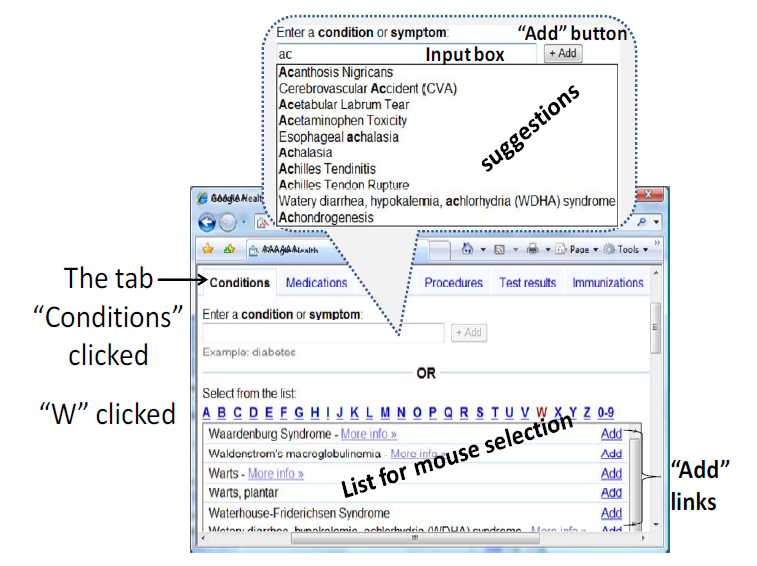
\includegraphics[width=0.7\textwidth]{fig/WebSideChannelExample1.png}
		\caption{Example Health Record System from \cite{WebSideChannel}}
		\label{Fig: HealthRecordSystem}
	\end{figure}
	
	In this example, the authors demonstrated that according to which tab or alphabet the user has clicked, the server returns a series of  packets with distinguishable lengths and directions. Further more, distinguishable packet traces can also be observed when user types in the input box triggering auto suggestion. As a result, an eavesdropper can deduce the user input simply by looking at the packet features of encrypted traffic.
\end{example}

\begin{example}
	The second vulnerable website is an online taxing service. In this system, the tax application form varies due to the payee's family status. The vulnerability of this website is that users are directed to different pages according to the form they are going to fill, while different pages results into packets of different lengths and directions, allowing an eavesdropper to reveal the family status of the user. The packet features of encrypted traffic again breached the data confidentiality.
\end{example}

%Financial charts Example
\begin{example}
	The third example is an online investment system where financial charts are provided to the users. The vulnerability is that an eavesdropper can distinguish which chart is presented to an user by the size of the chart which is a gif file. 
\end{example}

%Search Keyword Example (briefly, refers to the other one)
\begin{example}
	The last example shows how Traffic Analysis can be applied to attack the key word user provided to a search engine. \cite{SearchAttack} gives a more thorough description of this attack.
\end{example}

\cite{PinpointWeb} extends the work from a leakage detection perspective. Similar to \cite{WebSideChannel}, a web application is formally modelled as a state machine with user input and packet traces being the input and output respectively. The packet traces are aligned by sequence of packets. A hypothetical DETECT function is then iterated over all positions of aligned traces. For each position, DETECT function computes an information leakage metric and returns it as an indicator of potential information leakage at each position. The authors further instantiated the DETECT function by using Mutual Information of user input and packet features. Finally, they showed that in the experiment done on an example web application, the ACK flag could also be a potential leakage source in addition to packet sizes, where the latter is a widely exploited packet feature in many Traffic Analysis Attacks.

\cite{SearchAttack} implements the Traffic Analysis Attack on search engines described by \cite{WebSideChannel} in more details. It exploits the fact that Google by default enables auto suggestion which responds to each key stroke of user input with the suggest options and preloaded pages. This attack assumes the user input is within a finite dictionary. The attack is done in two steps:

\begin{enumerate}
	\item The first step is the profiling step. The attacker first builds a prefix tree\cite{PrefixTree} for the whole dictionary. Each edge of the prefix tree represents a key stroke from parent to child in the search box. The attacker associates each edges with the distribution of server responded packet sizes that is gathered through multiple trials. 
	\item When an user's traffic is captured, the attacker compares the sizes of server response for each user key stroke to the edges in the prefix tree of the corresponding depth. For each comparison, the attacker computes a likelihood and accumulates it through stochastic algorithms. 
\end{enumerate}

Finally, the algorithms outputs a set of keyword predicts of the highest likelihoods. At the end of the paper the authors showed that their method proved to be effective in their settings.

\subsubsection{Website Fingerprinting}
%Web site fingerprinting
Website Fingerprinting is a well studied topic in Traffic Analysis Attacks. \cite{WebsiteFingerprint} demonstrates the application scenario as in \Cref{Fig: Application Scenario of Website Fingerprint}. 

\begin{figure}[h!]
	\centering
	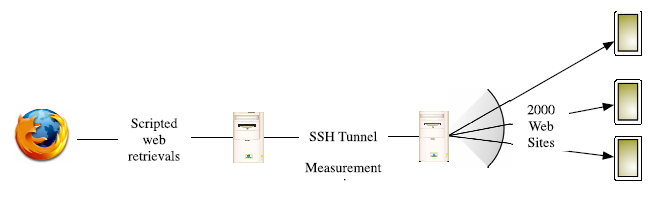
\includegraphics[width=0.7\textwidth]{fig/WebsiteFingerprint.png}
	\caption{Application Scenario of Website Fingerprint by \cite{WebsiteFingerprint}}
	\label{Fig: Application Scenario of Website Fingerprint}
\end{figure}

Tor\cite{Tor} can be considered as an instance of such network. The goal of Website Fingerprint is to identify the website an user is visiting through a secured channel by looking at the traffic features. Its motivation has received a growth in awareness in the cyber security community due to the recent years disputable governmental mass surveillance.

\cite{WebsiteFingerprint} demonstrates the use of machine learning techniques on packet sizes. To be more specifically, the authors conducted a series of experiment in a ``closed world'' setup of 2000 websites, i.e. assuming the user visits only one of 2000 known websites. To fingerprint a website, the attacker first visits the websites gathering the packet traces. These traces are then used as the training set and fed to the classifier. The captured user's traffic trace is then treated as the test set to predict which website the user has visited. Two classifier are tested in their experiments, namely Jaccard's coefficient and naive Bayes classifier. The results show that Jaccard's coefficient outperformed naive Bayes classifier in most cases. In addition, the authors also measure the affection of time elapsed and argued that these attacks still hold after 4 weeks of profiling. However, considering the fact that the nature of Internet has changed dramatically in the past decade, the last argument might need to be reconsidered.

%Peekaboo
A series of similar Website Fingerprint experiments has been studied by \cite{Peekaboo}, with aspect to the effectiveness of different countermeasures. Comparing to \cite{WebsiteFingerprint}, \cite{Peekaboo} analysed more packet features other than direction and length, including timing information, total bytes, total bytes on each direction, traffic bursts\footnote{A huge amount of traffic that has been transmitted continuously on the same direction.} and bandwidth. Classifiers from previous works are studied in this paper, namely LL classifier from \cite{WebsiteFingerprint}, H classifier from \cite{HClassifier} and P classifier from \cite{PClassifier}, alongside with some other classifiers designated to specific packet features. With respect to the countermeasures, different padding schemes are compared in this paper, including per packet padding, session wide padding and Traffic Morphing which is a sophisticated padding scheme we describe later in the context. In addition to padding schemes which mostly aimed to mitigate the packet length side channel, BuFLO\cite{Peekaboo} is also introduced to mitigate the timing and bandwidth side channels. For the result, the authors reported that all padding schemes above does not provide enough protection against the best classifier, i.e. the P classier. BuFLO does not bring much security neither unless used with a drastic overhead to the performance.

\subsubsection{Other Attacks on Different Applications}
%Apple iMessage
%SSH attack
%VoIP attack
%Skype Video
In spite of the attacks we mentioned above, there also exists many other Traffic Analysis Attacks against different applications on Internet. \cite{VoIPLanguage} and \cite{VoIPPhrases} demonstrated that the encrypted Voice over IP, VoIP, traffic could leak the language spoken and certain phrases can be detected. \cite{SSHKey} showed that user key stroke could be revealed by packet timing information. \cite{AppleMessage} shows that user's OS, message length, language and several behaviour can be identified through the size of encrypted packets. \cite{Video} showed that certain video event such as ambient change or object movement in a Skype video chat can be observed through the changes in packet features.

\subsection{Traffic Analysis Countermeasures}

Several countermeasures are proposed to mitigate Traffic Analysis Attacks. 

\subsubsection{Padding}

Padding is the most common countermeasure that intends to mitigate the packet size side channel. \cite{Peekaboo} summarised the most common padding schemes that aims to prevent Traffic Analysis Attacks. Notice that when a padding scheme would pad a packet longer than MTU, it is truncated to MTU instead.

\begin{description}[style=nextline]
	\item[Session Random Padding] 
	All packets in a session padded with the same random value of bytes.
	\item[Packet Random Padding]
	Each packet is padded with a random value of bytes.
	\item[Linear Padding]
	Each packet is padded to a multiple of 128 bytes.
	\item[Exponential Padding]
	Each packet is padded to the nearest power of 2.
	\item[Mice-Elephants Padding]
	Each packet is padded to either 128 or MTU.
	\item[Pad to MTU]
	Each packet is padded to MTU.
	\item[Packet Random MTU Padding]
	Each packet is padded to a random number selected uniformly between the data length and MTU.
\end{description}

Paddings are relatively easier to implement. However, the nature of constrained resources of WSN implies that paddings might not be appropriate due to their bandwidth overhead and thereupon more energy consumption.

\subsubsection{BuFLO}

Buffered Fixed Length Oubfuscator, BuFLO, is a countermeasure proposed in \cite{Peekaboo}. BuFLO is a ``fool-proof''\cite{Peekaboo} countermeasure that totally ignores the performance issues in practice and designed only to study at what level the Traffic Analysis Attacks can be mitigated in the setup of experiments in \cite{Peekaboo}. In general, BuFLO only sends identical length packets on a fixed frequency. Application data are queued in a buffer until either a packet is filled, or a timeout is reached and the data is sent along with padding. When no data is buffer, BuFLO sends dummy packets contains no application data. This countermeasure intuitively eliminates most of the packet features that could be exploited, but \cite{Peekaboo} reports that it does not achieve a satisfiable protection unless used with impractically huge performance  overhead (nearly 400\% in bandwidth).

\subsubsection{Traffic Morphing}

Traffic Morphing\cite{TrafficMorphing} is another countermeasure to Traffic Analysis Attacks. The idea is to mimic the distribution of packet features of one website to another. This is done through truncating or buffering packets and sending dummy packets by sampling from the target website. \cite{Peekaboo} reported this countermeasure outperformed the other padding schemes, although neither of them provides a satisfiable protection. This countermeasure is relatively easier to implement on TCP since TCP provides a reliable stream connection. When implementing Traffic Morphing on applications based on UDP, like most of WSN applications, the upper layer must handle the subtle transportation problems such as packet reordering and data segmenting. Although Traffic Morphing costs less overhead in bandwidth comparing to paddings, it is nevertheless unlikely to be adopted by WSNs as the constrained devices does not seem to be capable to afford the computation overhead of this countermeasure.

%HTTPOS
HTTPOS\cite{HTTPOS} is an implementation adopted this countermeasure. It is implemented on the client's  browser and manipulates the underneath TCP connection to control packet size, timing information, web object size and bandwidth. There are mainly two strategies adopted by HTTPOS:

\begin{description}[style=nextline]
	\item[The Diffusion Strategy]
	 Assuming the adversary uses a known training set, HTTPOS modifies the packet features to some value that has not appeared in the training set. \cite{HTTPOS} claims this strategy will force the adversary to random guess the website but this claim is some how contradictory to the concept of Machine Learning.
	\item[The Confusion Strategy]
	As of Traffic Morphing, HTTPOS modifies packet features by sampling from another website.
\end{description}

For the result, \cite{HTTPOS} reported that their approach achieved nearly perfect protection, i.e. the adversary's accuracy of correctly guessing a website has  dropped to nearly 0 in their test set. This is somehow contradictory to the results in \cite{Peekaboo}, even though the classifier are not exactly identical.

\subsubsection{Format Transforming Encryption}

To an extend, \cite{FTE} proposed a different approach that uses Format-Transforming Encryption, FTE, to circumvent Deep Packet Inspection,DPI, which is strongly related to Traffic Analysis Attacks. The general idea is to morph one type of traffic to another type of traffic, e.g. to morph encrypt SSH data to an ordinary HTTP request. Comparing to standard encryption and decryption, FTE additionally defines an Unrank function which encodes the ciphertext to the target format and a Rank function that decodes the ciphertext. FTE is interested in the Traffic Analysis aspect as it could potentially eliminate some packet features by transforming the original packet trace into a totally different packet trace.

\section{Methodologies in Information Leakage }

%There are many literatures discuss how to detect , quantify or exploit different types of side channel information leakage. 
In this section, we review a few of the methodologies that is developed to detect, exploit or quantify information leakage in different types of side channels. 

\subsection{Machine Learning}
%Different Classifiers
Machine Learning is a widely used technique in analysing information leakage in packet features such as \cite{Peekaboo} \cite{TrafficMorphing} \cite{WebsiteFingerprint} \cite{HClassifier} \cite{PClassifier} and \cite{HTTPOS} we have mentioned above. 

Typically, there are three steps in launching a Machine Learning based Traffic Analysis Attack:

\begin{enumerate}
	%Training set
	\item The adversary collects a set of traces containing the packet features with known secrets. The secret here means the type of information that the adversary attempts to attack, e.g. which website a trace corresponds to. This data set is the training set.
	%Classifier
	\item The training set is given as the input to an algorithm called classifier. The classifier reads the training set and eventually generates some rules that map the packet features to the secret. 
	%Test set
	\item The test set is the traces captured for the victim. The test set is analysed by the classifier which to produce guesses of the secrets.
\end{enumerate}

This procedure is a Supervised Learning in Machine Learning terminology.

%Configurable Parameters
Although most Machine Learning based Traffic Analysis Attacks adopts this similar strategy, there are certain configurable parameters that could greatly affect the outcome.

The first configurable is the packet features. Different classifier make use of different packet features, including headers, size and time of each packet and any connection level statistical features that can be computed through them. The adversary may select any subset of the packet features into the training set.

%Classifiers
The second configurable is the classifier. Classifiers are the core to the prediction. They vary in construction,  accuracy, performance and even inputs. We do not give the detailed explanation about the classifiers as it is beyond the scope of this report. 

\Cref{Tbl: Classifiers in Traffic Analysis Literatures} summarises the classifiers used in the literatures we mentioned in \Cref{Subsec: Traffic Analysis Attacks}

\begin{table*}[h!]
	\center
	\resizebox{\textwidth}{!}{%
	\begin{tabular}{|c|c|c|c|}
		\hline
		\textbf{Literature}                        & \textbf{Classifier}                                                        & \textbf{Input Packet Features}                                                                                                                                                                                                      & \textbf{Output Guess}                                             \\ \hline
		\cite{WebsiteFingerprint}, \cite{Peekaboo} & Naive Bayes                                                                & (Direction, Length)                                                                                                                                                                                                                 & Website                                                           \\ \hline
		\cite{WebsiteFingerprint}                  & Jaccard's                                                                  & (Direction, Length)                                                                                                                                                                                                                 & Website                                                           \\ \hline
		\cite{HClassifier}, \cite{Peekaboo}        & \begin{tabular}[c]{@{}c@{}}Multnominal Naive Bayes\\ (MNB)\end{tabular}    & (Direction,  Frequency Distribution of Length)                                                                                                                                                                                      & Website                                                           \\ \hline
		\cite{PClassifier}, \cite{Peekaboo}        & \begin{tabular}[c]{@{}c@{}}Support \\ Vector \\ Machine (SVM)\end{tabular} & \begin{tabular}[c]{@{}c@{}}(Direction, Length, Size Marker\cite{PClassifier}, \\ HTML Markers\cite{PClassifier}, Total Bytes, \\ Number Marker\cite{PClassifier}, \\ Percentage Incoming Packet, \\ Number of Packets)\end{tabular} & Website                                                           \\ \hline
		\cite{AppleMessage}                        & Naive Bayes                                                                & Length                                                                                                                                                                                                                              & \begin{tabular}[c]{@{}c@{}}User OS,\\  User Language\end{tabular} \\ \hline
		\cite{Peekaboo}                            & Naive Bayes                                                                & Total Time                                                                                                                                                                                                                          & Website                                                           \\ \hline
		\cite{Peekaboo}                            & VNG++                                                                      & \begin{tabular}[c]{@{}c@{}}Total Time, Total Per-Direction Bandwidth,\\ Traffic Burst\cite{Peekaboo}\end{tabular}                                                                                                                   & Website                                                           \\ \hline
	\end{tabular}
	}
	\caption{Classifiers in Traffic Analysis Literatures}
	\label{Tbl: Classifiers in Traffic Analysis Literatures}
\end{table*}

%Pros & Cons
Machine Learning is a practical and powerful way to detect information leakage over a combined set of side channel information and can be effectively applied in experiments. However, the drawback is that sometimes it is difficult to quantify the leakage by reversing the rules generated by the classifiers.

%Information Theoretic Approaches
\subsection{Information Theoretic Approaches} \label{Subsec: Information Theory}

Some other literatures studies information leakage from an Information Theoretic perspective. As explained earlier in \Cref{Subsec: Traffic Analysis Attacks}, \cite{PinpointWeb} detects information leakage using an Information Theoretic approach.

In Information Theory, Shannon entropy, abbreviate as entropy, is one of the most common metric that evaluates the uncertainty of a random variable. The entropy of a random variable $X$ is defined as $H(X)$:

\begin{equation} \label{Eq: Entropy}
	H(X) = - \sum_{x \in X}{P(x) \log{P(x)}}
\end{equation}

And the conditional entropy is defined as:
\begin{equation} \label{Eq: Conditional Entropy}
H(X|Y) = -\sum_{x \in X}\sum_{y \in Y}P(x,y)\log{P(x|y)}
\end{equation}

Higher $H(X)$ indicates higher uncertainty of $X$ and vice versa.

Information is therefore defined as the reduction of entropy. Intuitively, the less information we have with regard to the variable $X$, the more uncertain it is.

In case of side channel information leakage, we are mostly interested into the information of a secret variable $X$ that is contained in another observable variable $Y$. For example, information of cryptographic key contained in the power traces in Power Analysis Attacks\cite{DPA}, and information of website contents contained in packet features, etc. This concept is well captured by Mutual Information, defined as:

\begin{equation} \label{Eq: MI}
	I(X;Y) = H(X) - H(X | Y)
\end{equation}

\Cref{Eq: MI} can be intuitively interpreted as the reduction of the uncertainty of $X$ when given $Y$. As of this project, we are generally presuming the observable $Y$ to be any traffic feature we can observe in WSNs and $X$ any information of the upper layer application.

In practice, evaluating Mutual Information requires the prior distribution of $X$. This requirement in some scenarios cannot be met. For example as stated in \cite{PinpointWeb} where $X$ is the user input, the prior distribution may vary due to many factors such as different groups of user. Therefore as an alternative,  Capacity is used to evaluate the upper bound of information leakage over all prior distributions of $X$, i.e. the maximum Mutual Information over all possible prior distribution of $X$. The Capacity $C$ is formally defined as:

\begin{equation} \label{Eq: Capacity}
	C = \sup_{\forall P(X)}{I(X;Y)}
\end{equation}

where $\sup$ represents suprema and $\forall P(X)$ represents all possible distribution of $X$.

\cite{PinpointWeb} applies this strategy on each packet feature at each position of aligned packet traces. As stated in the paper, this method only detects potential leakage points\footnote{A packet feature at a specific position that leaks information.} but does not directly implies an attack. As a matter of fact, \cite{PinpointWeb} reports that TCP ACK packets is a potential leakage source but there is no known attacks that exploits this feature to our knowledge; instead, \cite{PClassifier} even excluded them from the traces considering them as a purely side effect of the protocol and thus irrelevant to the application data.

As stated by \cite{OneTryGuess}, it is showen by \cite{OneTryGuessOrigin} that mutual information does not cover the scenario which the adversary attempts to guess the secret in one try. Following this concept, \cite{OneTryGuess} quantifies the information leakage in a one trial guess scenario. For consistency, we use the notations revised in \cite{GLeakage}. 

\begin{definition}
	Suppose a secret value $x \in X$. Suppose $\pi$ the prior distribution of $X$ which is known by the adversary $\mathcal{A}$. The Prior Vulnerability $V(\pi)$ is defined as:
	
	\begin{equation}
		V(\pi) = \max_{x \in X}{\pi[x]}
	\end{equation}
	
	Suppose a channel $C$ which encodes $x \in X$ to an observable value $y \in Y$, that is
	
	\begin{equation}
		C[x,y] = P(y | x)
	\end{equation}
	
	The Posterior Vulnerability is then defined as:
	
	\begin{equation}
		V(\pi, C) = \sum_{y \in Y}{\max_{x \in X}{\pi[x]C[x,y]}} 
	\end{equation}
	
\end{definition}

Comprehensively, Prior Vulnerability is the best chance  $\mathcal{A}$ correctly guesses $x$ in one try. Posterior Vulnerability is the same probability but given the knowledge of $y$. 

\begin{definition}
	The vulnerabilities are converted to min-entropy by taking negative logarithm:
	
	\begin{eqnarray}
		\begin{aligned}
			H_{\infty}(\pi) &= -\log{V(\pi)} \\
			H_{\infty}(\pi) &= -\log{V(\pi,C)}
		\end{aligned}
	\end{eqnarray}
	
	Similar to Mutual Information, the min-leakage $L(\pi,C)$ is defined as the difference of vulnerabilities induced by $C$:
	
	\begin{equation}
		L(\pi, C) = H_{\infty}(\pi) - H_{\infty}(\pi, C)
	\end{equation}
	
	And corresponding min-capacity which is the worst case of leakage over all $\pi$:
	
	\begin{equation}
		ML(C) = \sup_{\pi}{L(\pi,C)}
	\end{equation}
\end{definition}

Remind that these definitions are defined to model the information leakage where the adversary attempts to guess the secret correctly in one try and hence model a binary scenario, i.e. the adversary either correctly guesses the secret or not. \cite{GLeakage} extends the model by introducing a hypothetical gain function $g$:

\begin{definition}
	The gain function $g(w,x)$ is defined as the advantage the adversary gains on a guess $w$ when the secret is $x$. $g(w,x)$ is constrained by $g(w,x) \in [0,1]$.
\end{definition}

An example of real world implication of gain function could be a Template Attack\cite{TemplateAttack} \cite{PracticalTemplate} where an incorrect but ``relevant'' guess can help the adversary to narrow down the key space.

Following the gain function, \cite{GLeakage} adapts the vulnerabilities to g-vulnerabilities $V_g$ by the advantage can gained by an adversary among all possible guesses $W$:

\begin{eqnarray}
	\begin{aligned}
		V_{g}(\pi) &= \max_{w \in W}\sum_{x \in X}{\pi[x]g(w,x)} \\
		V_{g}(\pi, C) &= \sum_{y \in Y}{\max_{w \in W}\sum_{x \in X}{\pi[x]C[x,y]g(w,x)}} \\
		&= \sum_{y \in Y}\max_{w \in W}\sum_{x \in X}P(x,y)g(w,x)
	\end{aligned}
\end{eqnarray}

And thereafter the g-entropy, g-leakage and g-capacity:

\begin{eqnarray}
	\begin{aligned}
		H_{g}(\pi) &= -\log{V_g(\pi)} \\
		H_{g}(\pi, C) &= -\log{V_g(\pi,C)}\\
		L_g(\pi, C) &= H_{g}(\pi) - H_{g}(\pi, C)\\
		ML_g(C) &= \sup_{\pi}{L_g(\pi,C)}
	\end{aligned}
\end{eqnarray}

Different types of leakage can be modelled by substituting different gain functions as described by \cite{GLeakage}. \cite{AddMulGLeakage} studies more algebraic properties of this model.

There are also other literatures study the improvements of these models. \cite{EstimateLeakage} proposed a method to estimate the information leakage with Mutual Information utilising Blahut-Arimoto algorithm\cite{Blahut}\cite{Arimoto}. \cite{Continuous} proposes the use of continuous instead of discrete variable to  better model some side channel information.

Comparing to Machine Learning, Information Theoretic methods provides more quantified details of leakage in theory. However, they are sometimes hard to perform due to practical reasons, such as computational power requirements.

%\subsection{Methods from other Side Channel Attacks}

%Correlation in DPA

%Timing Attack